\subsection{Global K-Means}
We have tested on each dataset 171 different configurations of the Global K-Means algorithm, by using the 3 different distance metrics with 19 different values of the k (from 2 to 20), and 3 different values for the number of buckets (2k, 3k and 4k). This time, we have only run the Global K-Means once for each of these configurations, since it is a deterministic algorithm that would return the same results every time. From the evaluation metrics extracted for each of these runs, we study the effect of each of the 3 hyperparameters and study the best performing runs according to each of the metrics.

\subsubsection{Hyperparameter Study}
As in the previous section, we start by observing some preliminary patterns about the effect of each hyperparameter on the clustering performance.

In Figure \ref{fig:globalkmeans:violin} we summarize the observed trends in each of the datasets (columns) for each of the hyperparameters (rows) with different metrics. It is not surprising to see that the patterns regarding the K-Means hyperparameters (k and distance metric) mostly repeat for the Global K-Means, since Global K-Means is mearly a modification of the same idea as the standard K-Means.

\begin{itemize}
    \item In the first row of plots, we observe that Hepatitis again favors low values of k; Mushroom does not achieve very conclusive results, but definitely gets consistently worse with higher values of k; and Pen-based benefits from intermediate values, getting more inconsistent for the highest ones.
    \item In the middle row, it is evident that the Clark distance performs significantly better on the Hepatitis dataset and significantly worse on the other 2 datasets, which are similar conclusions as we had reached before.
    \item In the last row, we observe that the clustering performance generally does not seem to be significantly altered by the different values of the number of buckets that we use to initilize the candidate points of the algorithm.
\end{itemize}


\begin{figure}[h]
    \centering
    \begin{tabular}{ccc}
        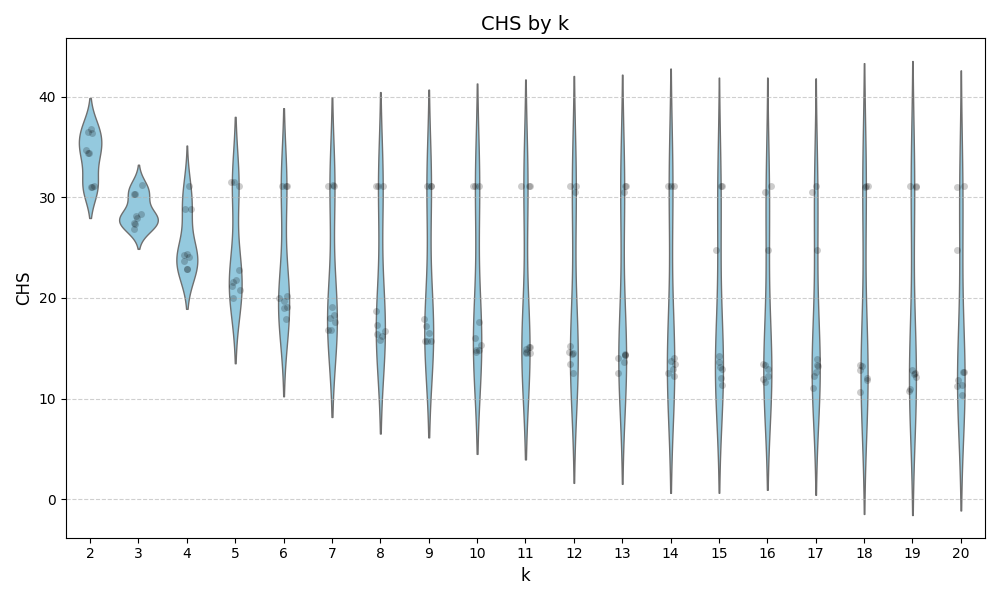
\includegraphics[width=0.3\textwidth]{figures/GlobalKMeans/hepatitis_violin_k_vs_CHS.png} & 
        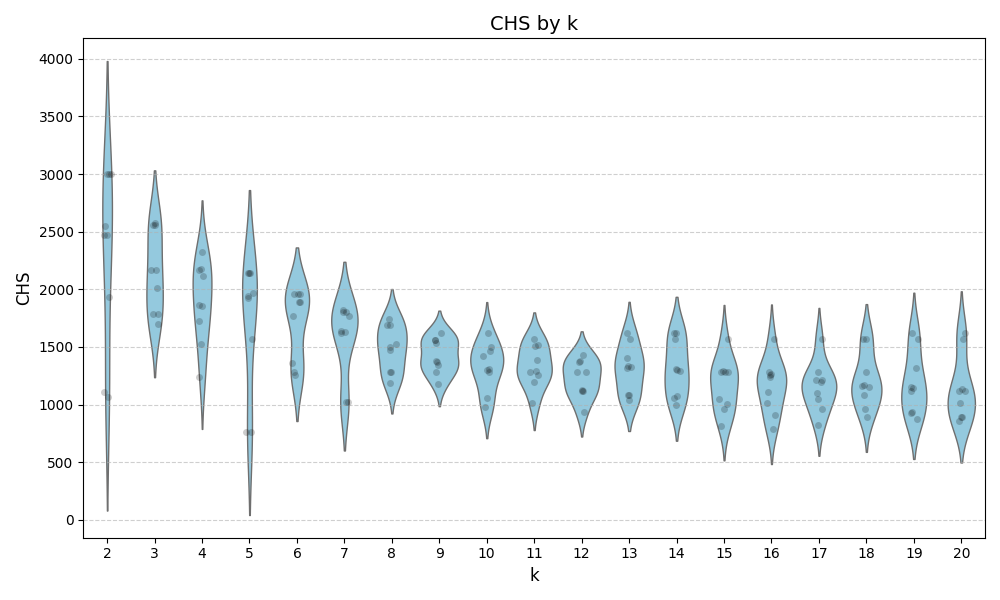
\includegraphics[width=0.3\textwidth]{figures/GlobalKMeans/mushroom_violin_k_vs_CHS.png} & 
        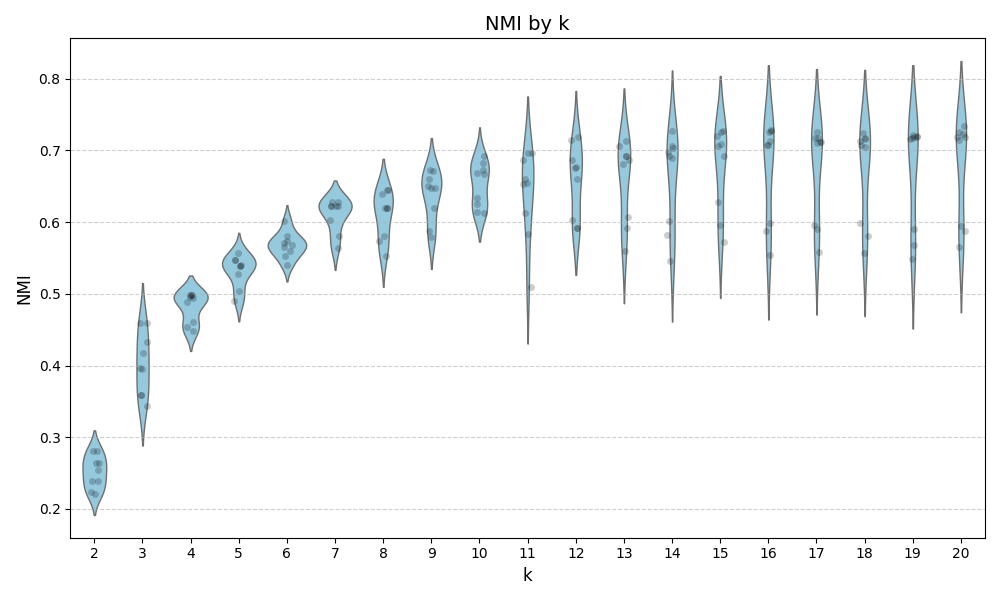
\includegraphics[width=0.3\textwidth]{figures/GlobalKMeans/penbased_violin_k_vs_NMI.png} \\
        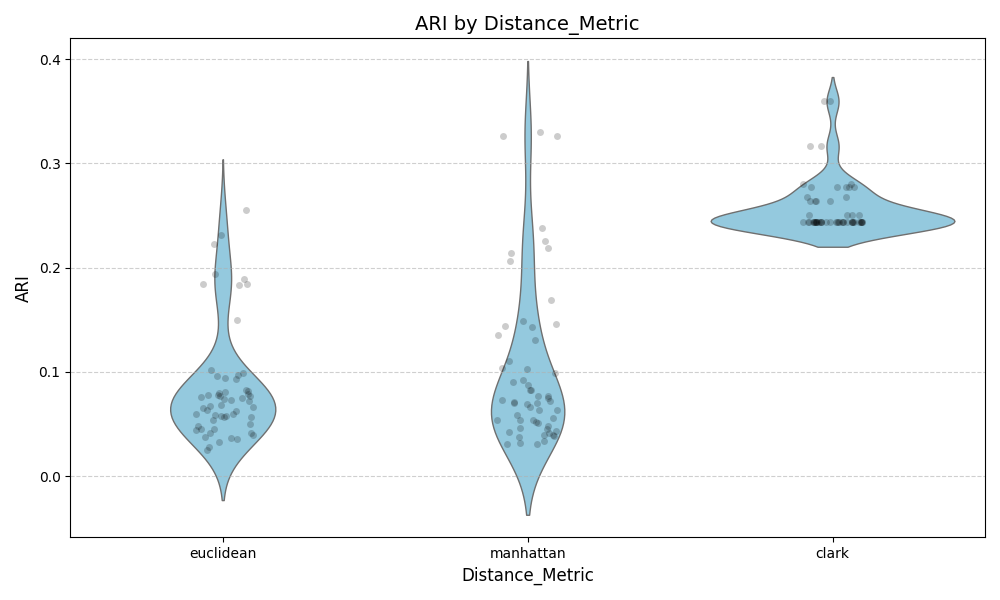
\includegraphics[width=0.3\textwidth]{figures/GlobalKMeans/hepatitis_violin_Distance_Metric_vs_ARI.png} & 
        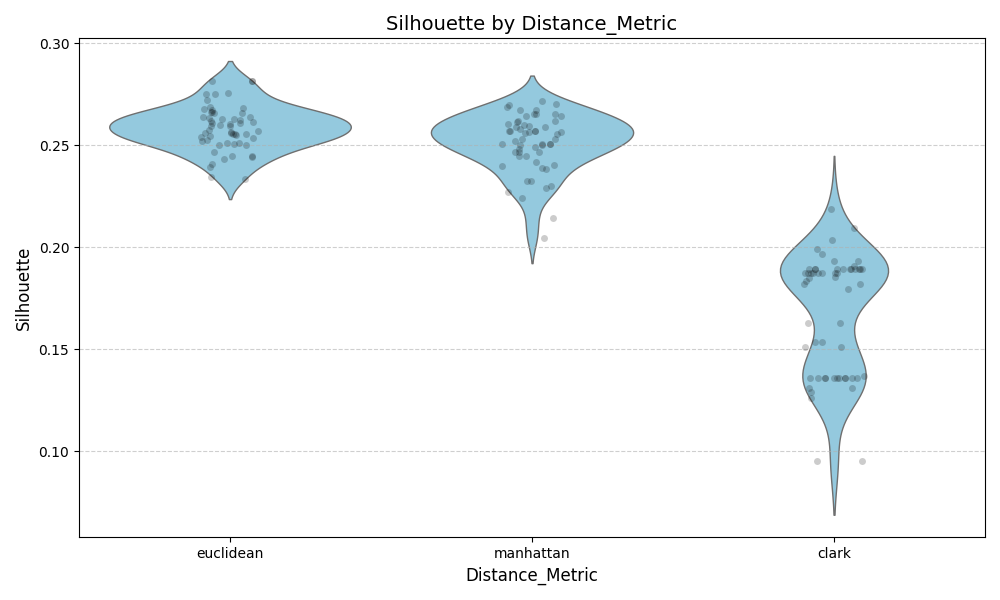
\includegraphics[width=0.3\textwidth]{figures/GlobalKMeans/mushroom_violin_Distance_Metric_vs_Silhouette.png} & 
        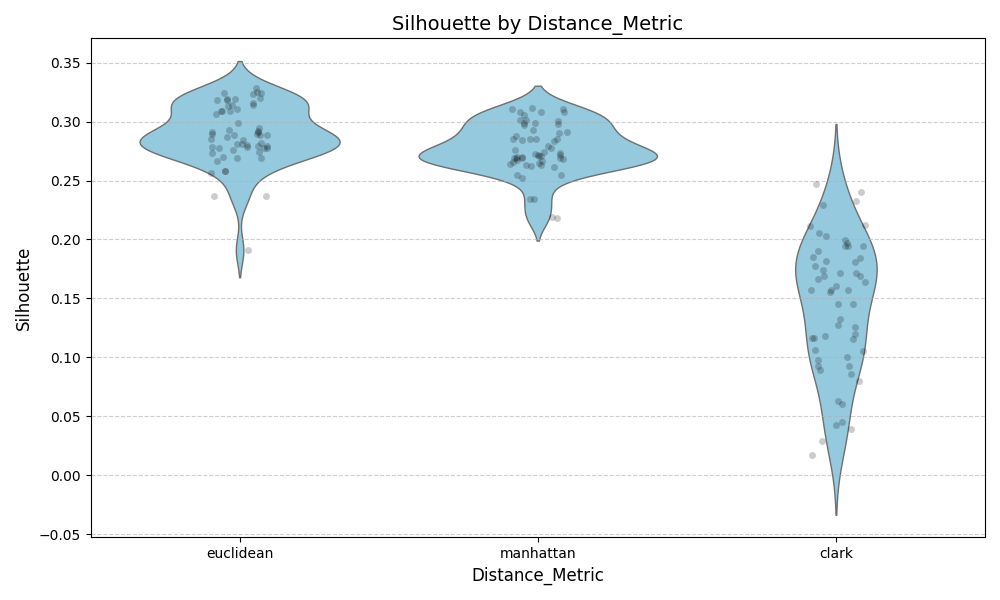
\includegraphics[width=0.3\textwidth]{figures/GlobalKMeans/penbased_violin_Distance_Metric_vs_Silhouette.png} \\
        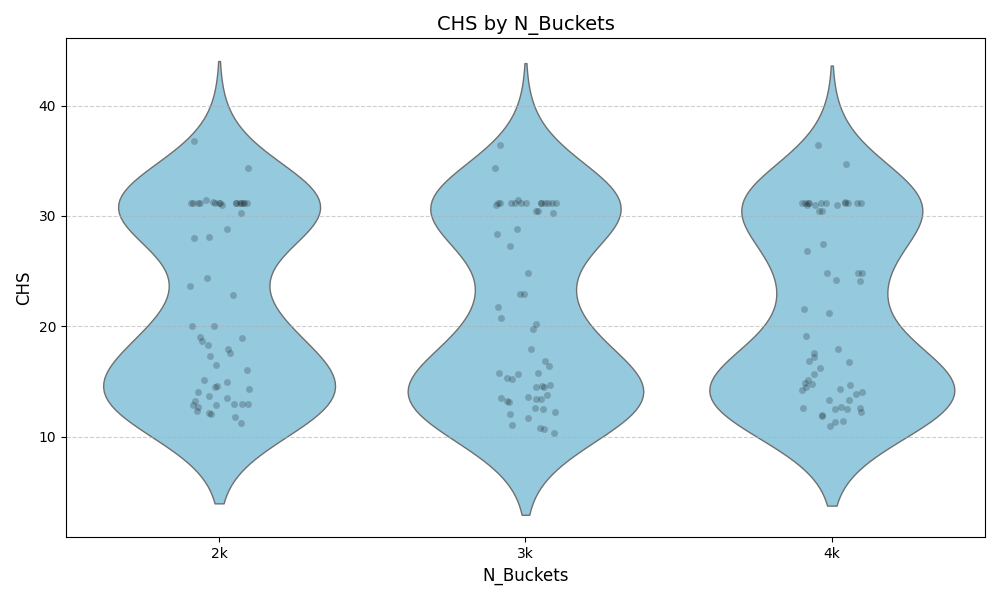
\includegraphics[width=0.3\textwidth]{figures/GlobalKMeans/hepatitis_violin_N_Buckets_vs_CHS.png} & 
        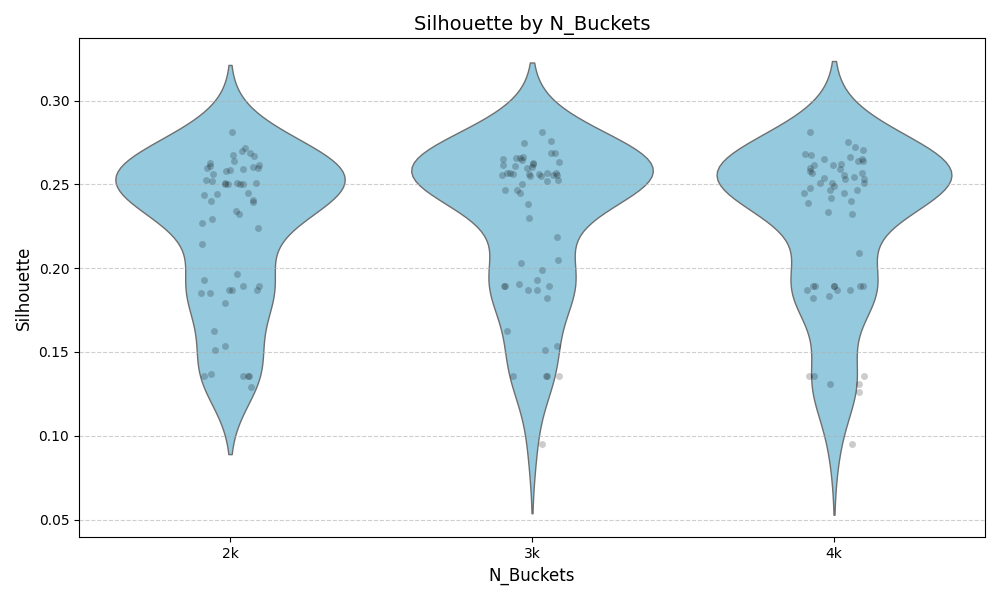
\includegraphics[width=0.3\textwidth]{figures/GlobalKMeans/mushroom_violin_N_Buckets_vs_Silhouette.png} & 
        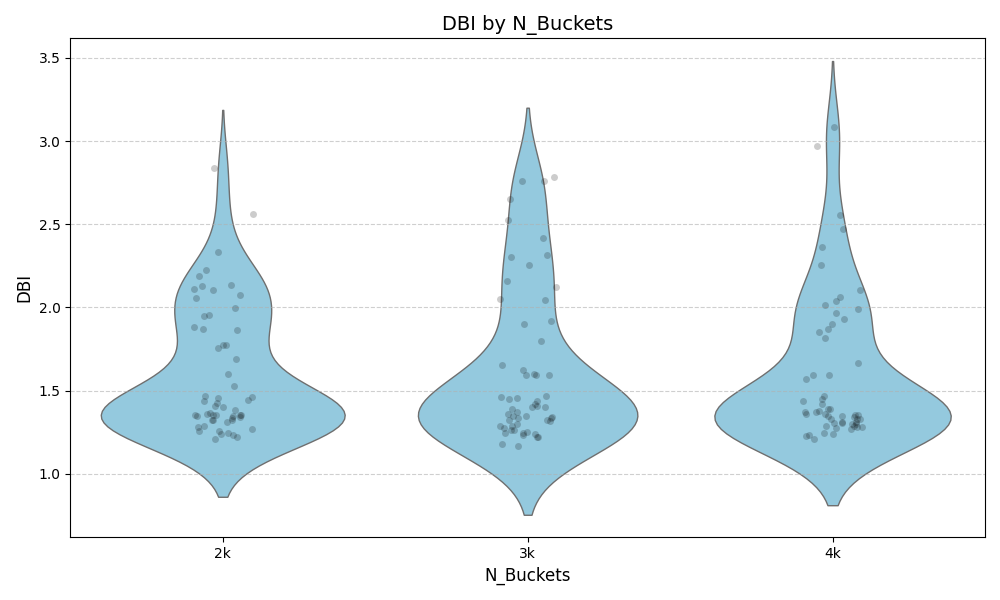
\includegraphics[width=0.3\textwidth]{figures/GlobalKMeans/penbased_violin_N_Buckets_vs_DBI.png} \\
    \end{tabular}
    \caption{Violin plots of the Global K-Means: Each row is a hyperparameter (k, distance metric, number of buckets), and each column is a dataset (Hepatitis, Mushroom, Pen-based)}
    \label{fig:globalkmeans:violin}
\end{figure}

\subsubsection{Best Runs}
As for the K-Means, we extracted for each of the datasets the run which achieved the best score for each of the metrics. A summary of them is displayed in Table \ref{tab:kmeans:best_runs}.

\textcolor{red}{TO DO}

\begin{table}[h!]
    \centering
    \begin{tabular}{|c|ccc|ccc|ccc|}
        \hline
                        & \multicolumn{3}{c|}{\textbf{Hepatitis}} & \multicolumn{3}{c|}{\textbf{Mushroom}} & \multicolumn{3}{c|}{\textbf{Pen-based}} \\ \hline
        \textbf{Metric} & \textbf{k} & \textbf{Distance} & \textbf{Value} 
                        & \textbf{k} & \textbf{Distance} & \textbf{Value} 
                        & \textbf{k} & \textbf{Distance} & \textbf{Value} \\ \hline
        ARI            & 2          & manhattan         & 0.37 
                       & 2          & clark         & 0.40 
                       & 14          & euclidean             & 0.64 \\ \hline
        NMI            & 3          & clark             & 0.25 
                       & 15          & clark         & 0.43 
                       & 14          & euclidean         & 0.74 \\ \hline
        DBI            & 20         & euclidean         & 1.40 
                       & 2         & euclidean             & 1.20 
                       & 7         & euclidean         & 1.23 \\ \hline
        Silhouette     & 2          & manhattan         & 0.21 
                       & 2          & euclidean         & 0.28 
                       & 10          & euclidean             & 0.32 \\ \hline
        CHS            & 2          & euclidean         & 36.77 
                       & 2          & euclidean         & 2996.24 
                       & 4          & euclidean         & 3361.02 \\ \hline
    \end{tabular}
    \caption{Metrics with corresponding values, k, and distance metrics for three datasets.}
    \label{tab:kmeans:best_runs}
\end{table}

From these results, we can make some deductions as to which are the best hyperparameter configurations of the K-Means for the 3 datasets:
\begin{enumerate}
    \item \textbf{Hepatitis:} It is again clear that low values of k (2 and 3) typically achieve better scores, which we had already observed before. On the other hand, it is not so clear which of the 3 distance metrics is more appropriate for this dataset, since all of them appear in the top scoring runs.
    \item \textbf{Mushroom:} We can observe once again that k=2 is dominant, probably due to the 2 classes that the dataset has. As for the distance metrics, Euclidean seems to be the most effective, followed by Clark, and Manhattan does not appear to be useful for the properties of this dataset.
    \item \textbf{Pen-based:} In this case, we do not see such a clear predominance of any specific value of k, but there seems to be a trend towards intermediate values, which was to be expected due to the 10 classes of the dataset. In contrast, we do see a constant primacy of the Euclidean distance metric over the rest, that clearly appears to be better at capturing key differences in this dataset than the other two.
\end{enumerate}
Additionally, we can observe that the 2 bigger datasets (Mushroom and Pen-based) have overall better top values of the metrics than the smaller, Hepatitis dataset. In particular, the Pen-based has the best results in all of the metrics except DBI (in which the difference is minimal), which leads us to the conclusion that it is the dataset for which the K-Means clustering algorithm is better suited.
